\documentclass[sigconf,anonymous,review]{acmart}

\usepackage{booktabs}
\usepackage{tabularx}
\usepackage{array}
\usepackage{enumitem}
\usepackage{tikz}
\usetikzlibrary{arrows.meta,positioning,shapes.geometric,fit}

\settopmatter{printacmref=true}
\acmConference[AISec '26]{19th ACM Workshop on Artificial Intelligence and Security}{October 2026}{TBD}
\acmBooktitle{19th ACM Workshop on Artificial Intelligence and Security (AISec '26)}
\acmYear{2026}
\copyrightyear{2026}
\acmDOI{}
\acmISBN{}

\newcommand{\system}{VCA prototype}
\newcommand{\vca}{verifiable containment attestation}

\begin{document}

\title{Verifiable Containment Attestation After LLM Guardrail Failure}

\author{Anonymous Author(s)}
\affiliation{\institution{Anonymous Institution}\country{}}

\begin{abstract}
LLM guardrails are commonly evaluated at the point where a user input is accepted or blocked. Agentic failures, however, can occur after this first gate has opened: untrusted retrieved content may gain authority, model output may request a tool, or unsafe text may be exported. This paper presents a provider-agnostic post-guardrail containment and evidence system. The prototype enforces input, context-provenance, tool-invocation, and output-leakage boundaries, then emits metadata-only evidence bundles signed with Ed25519 over canonical JSON. We evaluate the design through frozen corpora and signed evidence artifacts. On a 180-case reference corpus, 120 input-miss cases passed the input firewall and were downstream-contained, 30 direct-input attacks were blocked, and 30 benign hard negatives passed; targeted attack success was 0/150 on that corpus. A signed VCA bundle verifies offline and rejects tampering. In an observational input-only external-guardrail boundary study over the same frozen corpus, two recorded references---a generic external guardrail and a live Llama Guard 4 12B capture---missed 80 and 138 malicious cases respectively that the gateway then contained (80/80 and 138/138), with 0/150 targeted attack success in both. A public reproduction packet reports 12/12 tag-and-commit-pinned rungs with tiered replay depth. These results are bounded to the evaluated corpora and artifacts. They do not establish jailbreak immunity, production readiness, model safety, or vendor ranking.
\end{abstract}

\begin{CCSXML}
<ccs2012>
  <concept>
    <concept_id>10002978.10003029.10003032</concept_id>
    <concept_desc>Security and privacy~Systems security</concept_desc>
    <concept_significance>500</concept_significance>
  </concept>
  <concept>
    <concept_id>10010147.10010257.10010258.10010260</concept_id>
    <concept_desc>Computing methodologies~Artificial intelligence</concept_desc>
    <concept_significance>300</concept_significance>
  </concept>
</ccs2012>
\end{CCSXML}

\ccsdesc[500]{Security and privacy~Systems security}
\ccsdesc[300]{Computing methodologies~Artificial intelligence}
\keywords{LLM security, prompt injection, agentic systems, guardrails, attestation, reproducibility}

\maketitle

\section{Introduction}

Input guardrails are necessary, but they are not a complete security boundary for agentic LLM systems. A direct jailbreak may be visible in the user input. An indirect prompt injection may instead arrive through retrieved data, tool output, or model-generated text that is later interpreted as an action request. Prior work shows that LLM-integrated applications can treat untrusted data as instructions \cite{greshake2023indirect}; benchmark environments such as AgentDojo show that tool-using agents require explicit security evaluation under untrusted context \cite{debenedetti2024agentdojo}.

This paper studies a narrower systems question: after a guardrail misses, can a gateway produce machine-checkable evidence of what did and did not happen downstream? We do not propose a better jailbreak detector. We ask whether downstream containment can be made explicit, replayable, and cryptographically verifiable. The intended reader is a reviewer, operator, or auditor who should not have to trust a live service to know whether untrusted context gained authority, an unauthorized tool executed, or unsafe output was exported.

The \system{} enforces four boundaries: an input firewall, a context-provenance guard, a tool-invocation gate, and an output-leakage firewall. It treats model output and external guardrail verdicts as advisory. Each run emits metadata-only receipts and audit events. A second layer packages run-set evidence as canonical JSON and signs it with Ed25519 \cite{rfc8785,rfc8032}, using public verification keys and deterministic reproduction checks.

We make five contributions:
\begin{enumerate}[leftmargin=*]
  \item A containment model for evaluating downstream consequences after input guardrail misses.
  \item A provider-agnostic containment gateway with input, context-provenance, tool-invocation, and output-leakage boundaries.
  \item A \vca{} format: metadata-only canonical evidence bundles, Ed25519 signatures, public verification, offline reproduction, tamper rejection, and machine-readable non-claims.
  \item A reproducible evaluation ladder over frozen corpora and signed evidence, including a Fable-5-style reference containment regression, a signed VCA bundle, two external input-only guardrail reference runs, and a public reproduction chain.
  \item A claim-governance pattern that embeds non-claims and prevents bounded evidence from being converted into broad safety claims.
\end{enumerate}

\section{Background and Motivation}

Prompt injection is a first-order LLM application risk in practitioner guidance such as OWASP's LLM Top 10 \cite{owasp2025llmtop10}. The key distinction for this work is not whether prompt injection exists, but where it enters an agentic workflow. Direct injection targets the user turn. Indirect injection targets content later retrieved or processed by the application. Tool-using agents add a further boundary because model output can be interpreted as an action request unless a separate policy gate checks authorization.

Most guardrail evaluations report whether an input is blocked, warned, or allowed. That is useful, but it does not answer the downstream consequence question. If an input-only guardrail allows a benign-looking task while the malicious instruction lives in untrusted context, then the relevant security property is whether that context can gain authority. If a model asks to execute a tool, the relevant property is whether the tool request is authorized outside the model. If model output contains unsafe material, the relevant property is whether it reaches the export boundary.

The \system{} therefore treats containment evidence as the primary artifact. It records boundary outcomes without publishing raw harmful transcripts or raw model outputs. This evidence-first framing is also a reproducibility requirement: a reviewer should be able to verify the artifact offline, with public keys and scripts, rather than trusting a live provider or private deployment.

\section{Related Work}

\textbf{Prompt injection in LLM applications.} Indirect prompt injection showed that LLM-integrated applications blur the boundary between data and instructions: content retrieved from email, webpages, documents, or plugins can become operational instruction text once it reaches the model \cite{greshake2023indirect}. USENIX Security work has since formalized prompt-injection attacks and defenses, showing that case studies alone are insufficient and that defenses should be evaluated against explicit tasks, attack classes, and security properties \cite{liu2024formalizing}. Practitioner taxonomies, including OWASP LLM01, similarly separate direct and indirect injection and emphasize least privilege, output validation, human approval for high-risk actions, and segregation of untrusted content \cite{owasp2025llmtop10}. Our work follows this systems view but evaluates a different question: after the input guardrail misses, can downstream containment and its evidence be verified independently?

\textbf{Agent benchmarks and tool-use security.} AgentDojo evaluates LLM agents that operate tools over untrusted data and provides an extensible benchmark with realistic tasks, attacks, and defenses \cite{debenedetti2024agentdojo}. This line of work is essential for measuring whether agents complete tasks while resisting prompt injection. The VCA prototype is complementary: it does not claim a broad benchmark or a better attack detector. Instead, it records whether specific downstream consequences occurred, including context authority escalation, unauthorized tool execution, and unsafe output export, and then signs the evidence for offline verification.

\textbf{Guardrails and audit evidence.} Guardrails are usually evaluated as online decisions: input accepted, warned, or blocked. That frame is useful but incomplete for agentic systems because security-relevant outcomes can happen after acceptance. Our design borrows from security audit practice: preserve metadata, bind evidence with hashes and signatures, verify offline, and state non-claims. The use of canonical JSON and Ed25519 follows established standards for deterministic signing and verification \cite{rfc8785,rfc8032}. The novelty is not the cryptography itself; it is applying signed, machine-readable containment evidence to post-guardrail LLM security claims.

\section{Threat Model and Non-Claims}

The defender operates an agentic LLM gateway between user input, retrieved context, model output, tool execution, and final export. The assets are tool authority, confidential context, system/developer instructions, unsafe output surfaces, and the integrity of exported evidence. The adversary can submit direct prompt-injection text, place malicious instructions in untrusted context, cause unauthorized tool requests, attempt output leakage, and tamper with exported evidence after publication.

Out of scope are kernel compromise, malicious system operators, private-key theft, production deployment assurance, and formal proof of semantic safety. Signed evidence proves that an exported bundle was issued by the signing-key holder and was not modified after signing; it does not prove that the live service was uncompromised, that the signing key was never stolen, or that all possible attacks were covered. Table~\ref{tab:claims} records the main paper claims and their boundaries.

\begin{table*}[t]
\caption{Claims and non-claims. Evidence paths are repository-local and are verified in the paper package audit.}
\label{tab:claims}
\small
\begin{tabularx}{\textwidth}{p{0.28\textwidth}p{0.26\textwidth}X}
\toprule
Claim & Evidence source & Non-claim boundary \\
\midrule
Input-miss cases were downstream-contained on the frozen 180-case corpus & \texttt{stage-3l/metrics.json} & Does not imply general jailbreak resistance or production traffic validation. \\
The Stage 3M VCA bundle verifies offline and rejects tampering & \texttt{stage-3m/verifier-output.txt} and attestation files & Does not make signed evidence factual truth or prove the service was uncompromised. \\
The external guardrail captures are input-only boundary reference runs & \texttt{stage-3v/metrics.json}, \texttt{stage-3v-b/metrics.json} & Not a vendor ranking and not a model-safety proof. \\
The public VCA chain is replayable at tiered depths & \texttt{stage-3x/vca-chain-reproduction-results.json} & Not uniform 12/12 full reproduction. \\
\bottomrule
\end{tabularx}
\end{table*}

\section{System Design}

\begin{figure*}[t]
  \centering
  \resizebox{\textwidth}{!}{%
  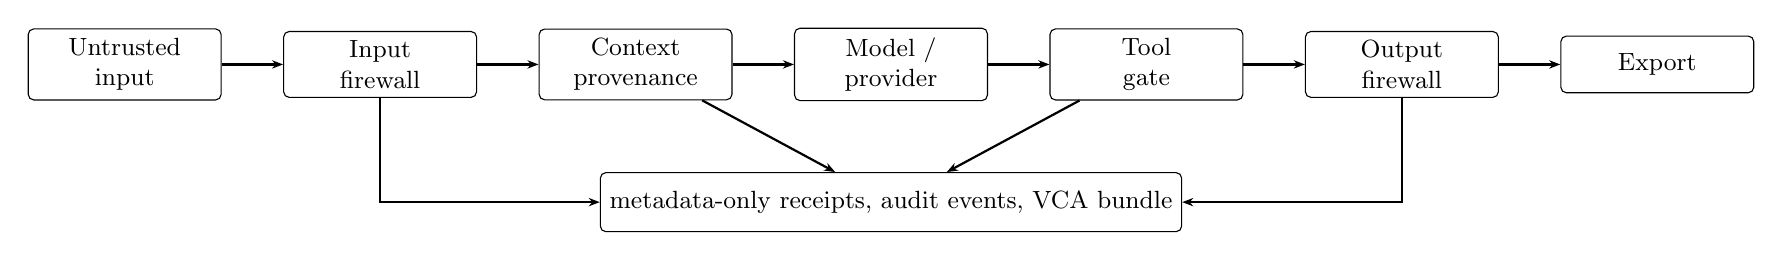
\begin{tikzpicture}[node distance=0.72cm and 0.78cm, box/.style={draw, rounded corners=2pt, align=center, minimum width=2.45cm, minimum height=0.72cm, font=\small}, wide/.style={draw, rounded corners=2pt, align=center, minimum width=5.4cm, minimum height=0.75cm, font=\small}, arr/.style={-{Stealth[length=4pt]}, thick}]
    \node[box] (input) {Untrusted\\input};
    \node[box, right=of input] (ifw) {Input\\firewall};
    \node[box, right=of ifw] (ctx) {Context\\provenance};
    \node[box, right=of ctx] (model) {Model /\\provider};
    \node[box, right=of model] (tool) {Tool\\gate};
    \node[box, right=of tool] (out) {Output\\firewall};
    \node[box, right=of out] (export) {Export};
    \node[wide, below=0.9cm of model] (evidence) {metadata-only receipts, audit events, VCA bundle};
    \draw[arr] (input) -- (ifw);
    \draw[arr] (ifw) -- (ctx);
    \draw[arr] (ctx) -- (model);
    \draw[arr] (model) -- (tool);
    \draw[arr] (tool) -- (out);
    \draw[arr] (out) -- (export);
    \draw[arr] (ifw) |- (evidence);
    \draw[arr] (ctx) -- (evidence);
    \draw[arr] (tool) -- (evidence);
    \draw[arr] (out) |- (evidence);
  \end{tikzpicture}}
  \caption{Post-guardrail containment pipeline. The defense acts after an input guardrail can fail. Provider output and external guardrail signals are advisory; final claims are derived from boundary evidence.}
  \Description{A pipeline from untrusted input through input, context, model, tool, output, and export stages, with evidence emitted from security boundaries.}
  \label{fig:pipeline}
\end{figure*}

Figure~\ref{fig:pipeline} shows the gateway. The input firewall handles direct attacks. If input passes, the context-provenance guard classifies each context item by origin and trust level; untrusted context can be passed as data but cannot acquire system or developer authority. Provider output is treated as untrusted material. Tool requests must pass the tool gate; final output must pass the output firewall before export. Table~\ref{tab:boundaries} summarizes each boundary, the attack class it addresses, its enforcement action, and the evidence it emits.

The design intentionally avoids using the model as its own security monitor. Boundary decisions are made by deterministic gateway code over structured metadata. The model and any external guardrail can influence the ordinary application response, but neither can authorize a tool, relabel untrusted context as trusted instruction, or suppress an audit event. This separation is what makes the later attestation meaningful: the evidence records gateway decisions rather than model assertions about those decisions.

\textbf{Evidence schema.} Each boundary emits a compact record with a run identifier, boundary name, policy version, input/output digests where applicable, verdict, reason code, and non-claim tags. Raw prompts and raw provider outputs are excluded from the evidence packet. The VCA bundle aggregates these records with corpus metadata, metric summaries, privacy reports, referenced evidence hashes, public verification metadata, and a machine-readable list of limitations. This lets a reviewer check both positive claims, such as ``no unauthorized tool execution in this corpus,'' and negative scope boundaries, such as ``not a production deployment claim.''

\begin{table*}[t]
\caption{Containment boundaries.}
\label{tab:boundaries}
\small
\begin{tabularx}{\textwidth}{p{0.18\textwidth}p{0.20\textwidth}p{0.28\textwidth}X}
\toprule
Boundary & Attack class & Enforcement action & Evidence emitted \\
\midrule
Input firewall & Direct prompt injection & Block or warn before provider call & Input verdict, receipt, audit event \\
Context provenance & Indirect prompt injection & Demote untrusted context to data & Context verdict and boundary label \\
Tool gate & Tool self-authorization & Refuse unauthorized request & Tool verdict and no-execution evidence \\
Output firewall & Leakage/export pressure & Block unsafe export & Output verdict and output hash metadata \\
\bottomrule
\end{tabularx}
\end{table*}

\section{Verifiable Containment Attestation}

\begin{figure}[t]
  \centering
  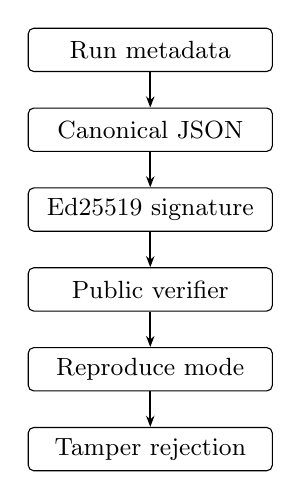
\begin{tikzpicture}[node distance=0.45cm, box/.style={draw, rounded corners=2pt, align=center, minimum width=3.1cm, minimum height=0.55cm, font=\small}, arr/.style={-{Stealth[length=4pt]}, thick}]
    \node[box] (run) {Run metadata};
    \node[box, below=of run] (json) {Canonical JSON};
    \node[box, below=of json] (sig) {Ed25519 signature};
    \node[box, below=of sig] (verify) {Public verifier};
    \node[box, below=of verify] (repro) {Reproduce mode};
    \node[box, below=of repro] (tamper) {Tamper rejection};
    \draw[arr] (run) -- (json);
    \draw[arr] (json) -- (sig);
    \draw[arr] (sig) -- (verify);
    \draw[arr] (verify) -- (repro);
    \draw[arr] (repro) -- (tamper);
  \end{tikzpicture}
  \caption{Evidence bundle and offline verification. The signature covers canonical parsed bundle content, not incidental formatting.}
  \Description{A vertical flow from run metadata to canonical JSON, signature, public verification, reproduction, and tamper rejection.}
  \label{fig:evidence}
\end{figure}

Figure~\ref{fig:evidence} shows the bundle and its offline verification flow. The attestation layer packages a run set as metadata-only evidence. A bundle contains metrics, boundary breakdowns, policy digests, privacy reports, referenced evidence hashes, and machine-readable non-claims. The signature covers canonical JSON, allowing a verifier to check the signed content independently of whitespace or formatting changes. Verification has a portable mode for schema, signature, digest, public-key fingerprint, referenced file hashes, gate results, and leakage scans. Reproduction mode reruns deterministic producers where available.

\section{Evaluation}

We use only repository evidence that can be traced to files and, where practical, commands. The evaluation ladder is shown in Figure~\ref{fig:ladder}; Table~\ref{tab:results} summarizes the main results and Table~\ref{tab:repro} the reproducibility and tamper checks.

\begin{figure}[t]
  \centering
  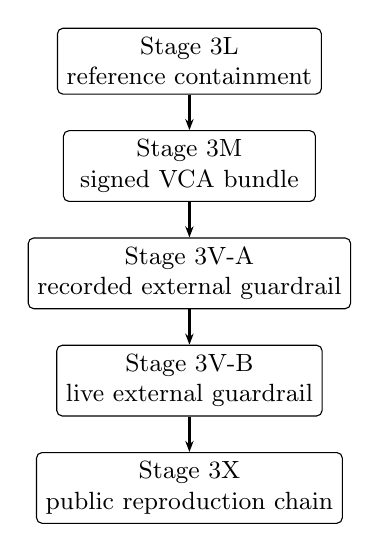
\begin{tikzpicture}[node distance=0.45cm, box/.style={draw, rounded corners=2pt, align=center, minimum width=3.2cm, minimum height=0.6cm, font=\small}, arr/.style={-{Stealth[length=4pt]}, thick}]
    \node[box] (l) {Stage 3L\\reference containment};
    \node[box, below=of l] (m) {Stage 3M\\signed VCA bundle};
    \node[box, below=of m] (va) {Stage 3V-A\\recorded external guardrail};
    \node[box, below=of va] (vb) {Stage 3V-B\\live external guardrail};
    \node[box, below=of vb] (x) {Stage 3X\\public reproduction chain};
    \draw[arr] (l) -- (m);
    \draw[arr] (m) -- (va);
    \draw[arr] (va) -- (vb);
    \draw[arr] (vb) -- (x);
  \end{tikzpicture}
  \caption{Evaluation ladder. Each stage contributes a different part of the paper claim and has a separate evidence artifact.}
  \Description{A vertical ladder of Stage 3L, Stage 3M, Stage 3V-A, Stage 3V-B, and Stage 3X.}
  \label{fig:ladder}
\end{figure}

\textbf{Stage 3L.} A deterministic 180-case corpus is driven through real gateway boundary functions in pipeline order: prompt classification, context-provenance checks, tool gating, and output scanning. The corpus contains 120 input-miss downstream cases, 30 direct-input attacks, and 30 benign hard negatives. The main dependent variables are consequence metrics: whether untrusted context gained authority, whether an unauthorized tool executed, whether unsafe output was exported, whether receipts were emitted, and whether the audit chain verified. To check that containment is not achieved by indiscriminate blocking, we also report a benign false-positive rate over the 30 hard negatives, all of which are adversarially shaped to resemble the malicious families while remaining legitimate; none were blocked (false-positive rate 0/30). This is a hard-negative control, not a full benign-traffic distribution.

Containment of the 120 input-miss cases is distributed across the downstream boundaries rather than concentrated at a single gate (Table~\ref{tab:ablation}): the context-provenance guard contained 72 cases, the tool gate 24, and the output firewall 24. The input firewall contained none of these by construction, because each input-miss case is designed to pass the input gate so that the downstream boundary under test is the one exercised.

\textbf{Stage 3M.} The Stage 3L run set is packaged into a metadata-only bundle signed with Ed25519. The public key and expected fingerprint are committed; the private key is not. The verifier checks structure, signature, evidence-file hashes, gate results, privacy, and reproduction matches. Tamper cases modify signed content, referenced metrics, and gate summaries to confirm that verification fails closed.

\textbf{Stage 3V-A.} To avoid resting the external-guardrail finding on a single point, we first use a recorded generic external guardrail as an independent advisory boundary over the same frozen 180-case corpus. It allowed 70 of 180 cases, blocked 70, and warned on 40; as an input-only signal its targeted attack success was 80/150. The gateway contained all 80 missed cases downstream (80/80), and external-plus-gateway targeted success was 0/150. This is a recorded observational point, not a live defense and not a ranking.

\textbf{Stage 3V-B.} A frozen live Llama Guard 4 12B capture provides a second, live advisory boundary point. The capture used \texttt{meta-llama/Llama-Guard-4-12B} in a single input-only greedy pass (temperature 0, 20 new tokens) under 8-bit quantization on one NVIDIA RTX 3090 24GB GPU, with transformers v4.51.3 Llama-Guard preview, PyTorch 2.8.0, and CUDA 12.8; the frozen capture, not the model, is replayed in CI. The model is not re-executed in CI. This is a boundary study, not a vendor comparison. The measured contrast is between an input-only advisory result and downstream gateway containment on the same frozen corpus. Table~\ref{tab:external} summarizes both external references.

\textbf{Stage 3X.} A public VCA timeline records tiered reproduction depth across 12 signed rungs.

\begin{table*}[t]
\caption{Main evaluation results.}
\label{tab:results}
\begin{tabularx}{\textwidth}{p{0.16\textwidth}p{0.24\textwidth}p{0.20\textwidth}p{0.15\textwidth}X}
\toprule
Evaluation & Corpus / evidence & Key metric & Result & Limitation \\
\midrule
Stage 3L & Frozen 180-case reference corpus & Input-miss downstream containment & 120/120 & Synthetic, redacted corpus only. \\
Stage 3L & Same & Direct-input attacks blocked & 30/30 & Does not imply general detector robustness. \\
Stage 3L & Same & Benign false-positive rate & 0/30 & Hard-negative control, not a full benign distribution. \\
Stage 3L & Same & Targeted attack success & 0/150 & Exact for corpus, not a world rate. \\
Stage 3L & Same & Unsafe tool/export/context escalation & 0/0/0 & Consequence metrics, not semantic safety proof. \\
Stage 3M & Signed VCA bundle & Offline verification & PASS & Signs evidence that exists; not factual truth. \\
Stage 3V-A & Recorded generic external guardrail & External misses contained & 80/80 & Recorded boundary point; no vendor ranking. \\
Stage 3V-B & Frozen live Llama Guard 4 capture & External misses contained & 138/138 & Input-only boundary study; no vendor ranking. \\
Stage 3X & Public reproduction packet & Rungs passed & 12/12 & Tiered replay, not uniform full reproduction. \\
\bottomrule
\end{tabularx}
\end{table*}

\begin{table*}[t]
\caption{External input-only guardrail references over the same frozen 180-case corpus. Each row is a recorded boundary point, not a vendor ranking. ``External-only'' counts the guardrail as the sole input gate; ``+ gateway'' adds downstream containment.}
\label{tab:external}
\small
\begin{tabularx}{\textwidth}{Xp{0.18\textwidth}p{0.16\textwidth}p{0.16\textwidth}}
\toprule
External guardrail (frozen) & External-only targeted ASR & Missed-but-contained & External + gateway ASR \\
\midrule
Recorded generic guardrail (3V-A) & 80/150 & 80/80 & 0/150 \\
Live Llama Guard 4 12B (3V-B) & 138/150 & 138/138 & 0/150 \\
\bottomrule
\end{tabularx}
\end{table*}

\begin{table*}[t]
\caption{Per-boundary containment of the 120 Stage 3L input-miss cases. The input firewall contains none by construction; each case is built to pass the input gate and exercise one downstream boundary.}
\label{tab:ablation}
\small
\centering
\begin{tabular}{lr}
\toprule
Downstream boundary & Input-miss cases contained \\
\midrule
Context-provenance guard & 72 \\
Tool gate & 24 \\
Output firewall & 24 \\
\midrule
Total downstream-contained & 120 \\
\bottomrule
\end{tabular}
\end{table*}

\begin{table*}[t]
\caption{Reproducibility and tamper checks.}
\label{tab:repro}
\small
\begin{tabularx}{\textwidth}{p{0.20\textwidth}p{0.16\textwidth}p{0.16\textwidth}X}
\toprule
Check & Expected & Verified & Command / source \\
\midrule
Stage 3M verifier & PASS & PASS & \texttt{stage-3m/verifier-output.txt} \\
Evidence leakage & zero & true & Stage 3M verifier output \\
Bundle digest & match & true & Stage 3M verifier output \\
Stage 3X timeline & PASS & true & \texttt{vca-chain-reproduction-results.json} \\
Tier summary & 3 reproduce, 7 hash, 2 index & matched & Stage 3X results JSON \\
\bottomrule
\end{tabularx}
\end{table*}

\section{Security Analysis}

The system prevents a bounded class of downstream consequences in the evaluated corpora: untrusted context gaining authority, unauthorized tool execution, and unsafe output export. It does so by separating model text from policy authority. The evidence layer makes the resulting containment claim checkable offline.

The system does not prove semantic harmlessness. An attacker outside the threat model could compromise the signing key, the host, or the evidence producer. A malicious operator could choose not to record evidence. A broader real-world deployment would also need operational key management, monitoring, and incident response. These are deployment concerns outside the paper's research prototype claim.

\section{Ethics and Responsible Release}

This is defensive research. The paper and artifact avoid releasing raw harmful jailbreak transcripts or operational payloads. The corpora are synthetic or redacted. The evidence is metadata-only and omits raw prompts, raw provider outputs, private keys, and real user data. The external guardrail study is vendor-neutral and must not be read as a ranking. The prototype is not deployment-ready or compliance-approved. These boundaries are stated in the paper, source notes, and artifact README.

\section{Limitations and Future Work}

The main external-validity limitation is that the evaluation uses frozen synthetic corpora and replay artifacts, not production traffic. The live model capture origin is self-reported and signed into evidence, but the verifier does not rehash model weights or prove the original GPU environment. Stage 3X reports uneven replay depth; this is honest, but it means the public chain is not uniformly fully reproduced. Future work should include third-party artifact evaluation, broader public benchmarks, deployment key-management analysis, and independent replication on additional agent stacks.

\section{Conclusion}

Input guardrails will sometimes miss. The \system{} evaluates and attests what happened downstream after the miss: whether untrusted context gained authority, whether unauthorized tools executed, whether unsafe output was exported, and whether the evidence verifies offline. The contribution is not jailbreak immunity. It is a bounded systems pattern for converting post-guardrail containment from a verbal assurance into a machine-checkable artifact.

\bibliographystyle{ACM-Reference-Format}
\bibliography{references}

\section*{Generative AI Usage}

Generative AI tools were used as writing and engineering assistants during development and drafting. The authors remained responsible for all claims, experiments, code review, evidence interpretation, and final manuscript content. No confidential peer-review material was shared with AI tools.

\end{document}
